\documentclass[cjk]{beamer}
\usetheme{UIBK} %Standard UIBK Template
\usefonttheme[onlymath]{serif}

\usepackage[utf8]{inputenc}
\usepackage{tikz}
\usepackage{listings}
\definecolor{mygreen}{rgb}{0,0.6,0}
\definecolor{mygray}{rgb}{0.5,0.5,0.5}
\definecolor{mymauve}{rgb}{0.58,0,0.82}
\definecolor{bggray}{rgb}{0.93,0.95,0.94}

\lstset{ %
backgroundcolor=\color{bggray},      % choose the background color
columns=fullflexible,
tabsize=4,
breaklines=true,               % automatic line breaking only at whitespace
captionpos=b,                  % sets the caption-position to bottom
commentstyle=\color{mygreen},  % comment style
escapeinside={\%*}{*)},        % if you want to add LaTeX within your code
keywordstyle=\color{blue},     % keyword style
stringstyle=\color{mymauve}\ttfamily,  % string literal style
frame=shadowbox,
rulesepcolor=\color{red!20!green!20!blue!20},
% identifierstyle=\color{red},
language=c++,
numbers=left,
numberstyle=\tiny\sffamily,
basicstyle=\tiny\ttfamily,% size of fonts used for the code
escapeinside=``,
xleftmargin=0.6em,
xrightmargin=0.6em,
aboveskip=1em
}
\usepackage{fontenc}
\usepackage[]{xeCJK,fontspec}
\setCJKmainfont{FandolSong}%{SimSun}
\setmainfont{CMU Serif}
\setsansfont{CMU Sans Serif}
\setmonofont{Sarasa Fixed SC}
%\setCJKmainfont{叶根友疾风劲草}
\setCJKfamilyfont{song}{FandolSong}
\newcommand{\song}{\CJKfamily{song}}
\setCJKfamilyfont{kaiti}{FandolKai}
\newcommand{\kaiti}{\CJKfamily{kaiti}}
\setCJKfamilyfont{heiti}{FandolHei}
\newcommand{\heiti}{\CJKfamily{heiti}}
%\usefonttheme[onlymath]{serif}
\usepackage{indentfirst}

\usepackage{graphics,tcolorbox}
\usepackage{graphicx,xcolor,xcolor-solarized}
\usepackage{amsmath,amssymb,amsfonts}
%\usepackage{manfnt}
\newcommand{\chuhao}{\fontsize{42pt}{\baselineskip}\selectfont}

\mode<article> % 仅应用于article版本
{
  \usepackage{beamerbasearticle}
  \usepackage{fullpage}
  \usepackage{hyperref}
}

\usefoottemplate{\vbox{%
\tinycolouredline{structure!120}%
 {\color{white}\textbf{\insertshortauthor\hfil%
 \insertshorttitle}\hfil   \insertframenumber{} / \inserttotalframenumber}%\hfil
}}
\makeatother
\newtheorem{原因}{{原因}}[section]
\newtheorem{定义2.2}{{定义2.2}}[section]
\newtheorem{引理2.1}{{引理2.1}}[section]
\newtheorem{引理2.2}{{引理2.2}}[section]
\newtheorem{定理2.1}{{定理2.1}}[section]
\newtheorem{定理2.2}{{定理2.2}}[section]
\newtheorem{为什么追求高精度?}{{为什么追求高精度?}}[section]
%\newtheorem{definition}{{definition}}[section]
\newtheorem{lem}{{引理}}[section]
\newtheorem{remark}{{注记}}[section]
\newtheorem{dingyi}{{定义}}[section]
\renewcommand{\figurename}{图}
%\usepackage[default]{comfortaa}

\author{组员:仇琨元\ 徐嘉睿\ 肖锐卓\ 吴雨飞}
\title{Matrix Multiplication Acceleration}
\subtitle{Implemented By Strassen Algorithm and Intel(R) Math Kernel Library}
\institute{Insitute of EEE \\ SUSTC}
\date{\today}

\begin{document}

%titlepage without header/footer and framenumbering
\begin{frame}[plain]
  \titlepage
\end{frame}

\begin{frame}{Contents}
  \tableofcontents
\end{frame}


%show table of contents at the beginning of every section
\AtBeginSection[]{
  \begin{frame}<beamer>
    \frametitle{Contents}
    \tableofcontents[currentsection]
  \end{frame}
}

\begin{frame}{Itemize}
  \frametitle{{\small Necessity of Matrix Multiplication Acceleration}}
  \begin{enumerate}
    \normalsize

    %     \item \href{./figure/com.pdf}{导心系统回顾}\\
    \item \textbf{Background}\\
          {\tiny Necessity of Matrix Multiplication Acceleration}\\
          \qquad\\
    \item \textbf{Therotical Analysis}\\
          {\tiny Strassen Multiplication}\\
          {\tiny AVX2 Instruction Set}\\
          \qquad\\
    \item \textbf{Methodology}\\
          {\tiny Strassen Method}\\
          {\tiny Intel(R) MKL BLAS Level 3 Routines}\\
          \qquad
    \item \textbf{Experiment Results}\\
          {\tiny Naive Matrix Multiplication}\\
          {\tiny Strassen Matrix Multiplication Without Minimun Size}\\
          {\tiny Strassen Matrix Multiplication with Minimun Size}\\
          {\tiny MKL Accelerated Strassen Algorithm}
          \qquad\\
    \item \textbf{Acknowledgements}\\
          %   \item \href{./figure/Boris.pdf}{Boris algorithm 数值算例}\\%3
          %     \qquad\\
          %     \item Boris algorithm 是否是共轭辛的\\%1:系统本身的稳定性:研究系统本身的性质,找出稳定的区域
          %数值格式的稳定性:有效控制计算过程中数据大小,使其再有限步计算中范数相对有界\\
  \end{enumerate}
  %     \tableofcontents
\end{frame}

\section{Background}
\begin{frame}
  \frametitle{\textbf{Necessity of Matrix Multiplication Acceleration}}
  \vspace{5mm}
  \small
  ~~~~The multiplication of two matrices is one of the most basic operations of linear algebra and scientific computing.

  ~~~~Modern signal processing, artificial intelligence and computer vision are all based on the fast and accurate algorithm of matrix multiplication, LU/QR/SVD decomposition and many other operations.

\end{frame}
\begin{frame}
  \frametitle{\textbf{Comparison of the time costs of computing the FFT}}

  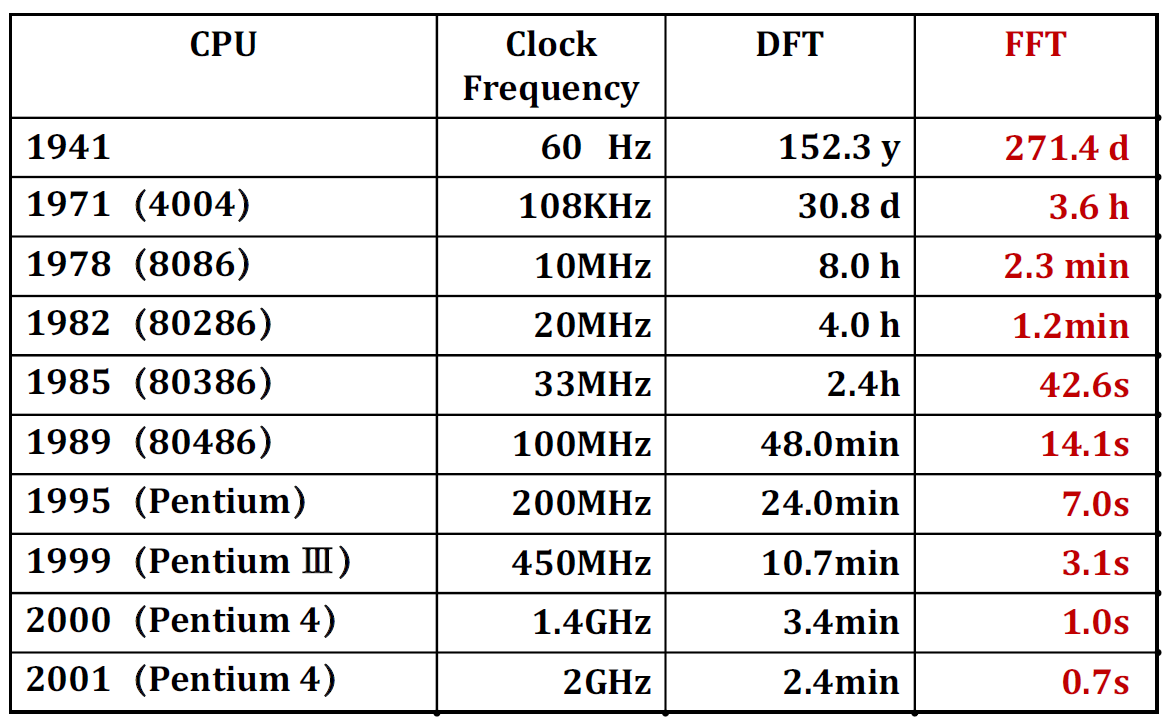
\includegraphics[height=5.0cm]{fftvel.png}

\end{frame}


\section{Therotical Analysis}
\subsection{Strassen Algorithm}
\begin{frame}[fragile]
  \frametitle{\textbf{Brute-Force Algorithm}}
  ~~~~The Strassen Multiplication uses divide-conquer to reduce the time complexity of MM operations.
  Normal MM uses 3 nested loops to perform the vector dotting and traversal of the rows and columns of the 2 operands:
  \begin{lstlisting}
    STANDARD-MATRIX-MULTIPLY (A,B):
    let C be a new m*n matrix
      for i <- 1 to m
        for j <- 1 to n
          C[i,j] = 0
            for k = 1 to p
                C[i,j] += A[i,k]*B[k,j]
      return C
  \end{lstlisting}
\end{frame}
\begin{frame}
  \frametitle{\textbf{Brute-Force Algorithm}}

  From the pseudocode above, let MUL, ADD and READ refers the \(assembly\) commands of the computer.
  Each nested loop multiplies the time complexity by its iteration number:
  \begin{equation}
    \begin{aligned}
      T(\text{Naive})                  & =m\cdot n\cdot p\cdot (T(\text{MUL}+\text{ADD}+2\text{READ})) \\
                                       & =\Theta(mnp)                                                  \\
      m=n=p\Rightarrow T(\text{Naive}) & =\Theta(n^{3})
    \end{aligned}
  \end{equation}

\end{frame}
\begin{frame}[fragile]
  \frametitle{\textbf{Strassen Algorithm}}
  Pseudocode of the Strassen algorithm:
  \begin{lstlisting}
    STRASSEN (MatrixA,MatrixB)
        N=MatrixA.rows
      Let MatrixResult be a new N×N matrix
      if N==1
        MatrixResult=MatrixA*MatrixB
      else
         // DIVIDE: partitioning input Matrices into 4 submatrices each
           for i  <-  0  to  N/2
               for j  <-  0  to  N/2
                  A11[i][j]  <-  MatrixA[i][j]
                  A12[i][j]  <-  MatrixA[i][j + N/2]
                  A21[i][j]  <-  MatrixA[i + N/2][j]
                  A22[i][j]  <-  MatrixA[i + N/2][j + N/2]

                  B11[i][j]  <-  MatrixB[i][j]
                  B12[i][j]  <-  MatrixB[i][j + N/2]
                  B21[i][j]  <-  MatrixB[i + N/2][j]
                  B22[i][j]  <-  MatrixB[i + N/2][j + N/2]
  \end{lstlisting}
\end{frame}
\begin{frame}[fragile]
  \frametitle{Strassen Algorithm}
  \begin{lstlisting}
  // CONQUER: here we calculate P1...P7 matrices
      P1 <- STRASSEN(A11, B12-B22)          //P1=A11(B12-B22)
      P2 <- STRASSEN(A11+A12, B22)          //P2=(A11+A12)B22
      P3 <- STRASSEN(A21+A22, B11)          //P3=(A21+A22)B11
      P4 <- STRASSEN(A22, B21-B11)          //P4=A22(B21-B11)
      P5 <- STRASSEN(A11+A22, B11+B22)      //P5=(A11+A22)(B11+B22)
      P6 <- STRASSEN(A12-A22, B21+B22)      //P6=(A12-A22)(B21+B22)
      P7 <- STRASSEN(A11-A21, B11+B12)      //P7=(A11-A21)(B11+B12)

        // calculate the result submatrices
      C11  <-  P5 + P4 - P2 + P6
      C12  <-  P1 + P2
      C21  <-  P3 + P4
      C22  <-  P5 + P1 - P3 - P7

        // MERGE: put them together and make our resulting Matrix
      for i  <-  0  to  N/2
         for j  <-  0  to  N/2
           MatrixResult[i][j]              <-  C11[i][j]
           MatrixResult[i][j + N/2]        <-  C12[i][j]
           MatrixResult[i + N/2][j]        <-  C21[i][j]
           MatrixResult[i + N/2][j + N/2]  <-  C22[i][j]
      return MatrixResult
\end{lstlisting}
\end{frame}
\begin{frame}
  \frametitle{Strassen Algorithm}

  Use the recursion function to evaluate the time complexity of the algorithm.
  For \(n\geqslant 2\),
  \begin{equation}
    \begin{aligned}
      T(2n)                          & =7T(n)+\Theta(n^{2})              \\
      \log_{2} n=k\Rightarrow T(k+1) & =7T(k)+\Theta(2^{2k})             \\
      \Rightarrow T(n)               & =O(n^{\log_{2}7})                 \\
                                     & \approx O(n^{2.81})<\Theta(n^{3})
    \end{aligned}
  \end{equation}
\end{frame}


\subsection{Intel MKL}
\begin{frame}
  \frametitle{Intel Math Kernel Library}

  \begin{figure}[htb]
    \begin{center}
      
\includegraphics[height=5.0cm]{yagao-logo.jpg}
    \end{center}
  \end{figure}

\end{frame}
\begin{frame}
  \frametitle{Intel Math Kernel Library}

  The \textbf{MKL} is a optimized implementation of many math functions exclusively on x86 architecture and processors supports the Intel SIMD instructions, especially in Intel(R) processors. This library is implemented by assembly codes and C++ codes that are extremely optimized by Intel SIMD instructions(\textbf{SSE},\textbf{AVX}), in order to maximize performance on matrix operations.

\end{frame}
\begin{frame}
  \frametitle{Performance of Intel MKL}
  The Intel MKL computes the 2500*2500 matrix multiplication within 6000 milliseconds.
  \begin{figure}[htb]
    \begin{center}
      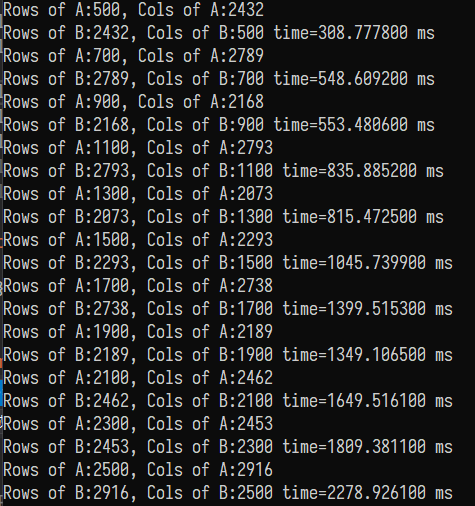
\includegraphics[height=5.0cm]{mkl_dgemm.png}
    \end{center}
  \end{figure}

\end{frame}

\section{Methodology}
\begin{frame}{Blocks}
  \begin{block}{Lorem Ipsum}
    Lorem ipsum dolor sit amet, consetetur sadipscing elitr, sed diam nonumy eirmod tempor invidunt ut labore et dolore magna aliquyam erat, sed diam voluptua.
    At vero eos et accusam et justo duo dolores et ea rebum. Stet clita kasd gubergren, no sea takimata sanctus est Lorem ipsum dolor sit amet.
  \end{block}
  \begin{block}{Observation}
    Simmons Dormitory is composed of brick.
  \end{block}
\end{frame}


\section{Experiment Results}
\begin{frame}{OCaml Code}
  \begin{center}
    \begin{block}{Paragraph function}
      Write a function 'paragraph' that constructs a picture of width w of some text t, such that the content splits into as many lines as needed to fit into a paragraph of w columns.
    \end{block}
    \begin{block}{paragraph.ml}
      {\small  \lstinputlisting[language=ml]{src/paragraph.ml}  }
    \end{block}
  \end{center}
\end{frame}


%final slide
\begin{frame}[plain,noframenumbering]
  \begin{beamercolorbox}[wd=\paperwidth, ht=1.4cm,rounded=true,shadow=true]{final slide}
    \begin{center}
      {\huge Thank you for your attention!}
    \end{center}
  \end{beamercolorbox}
\end{frame}

\section{Acknowledgements}
\begin{frame}[noframenumbering]{Backup-Slide}
\end{frame}


\end{document}
